\documentclass{article}
%\setlength{\mathindent}{0pt}
% Package for better handling of figures
\usepackage{graphicx}
% Package for better handling of tables
\usepackage{array}
% Package for better handling of mathematical symbols
\usepackage{mathrsfs}
\usepackage{amsmath}
\usepackage{amssymb}
\usepackage{multirow}
\usepackage{array}
\usepackage{float}
\usepackage{algorithm}
\usepackage{algpseudocode}


% Title and Author Information
\title{Privacy-Preserved Meeting Organization}
\author{Group 06}
\date{\today} % You can specify a different date if needed

\begin{document}

% Title Page
\maketitle

% Tentative basic definitions
\section{Basic definitions}

\noindent
Following finite sets are defined:
\begin{itemize}
    \item $\mathcal{D}$: The set of all documents.
    \item $\mathcal{R}$: The set of all roles.
    \item $\mathcal{I}$: The set of all individuals
    \item $\mathcal{L}$: The set of all locations.
    \item $\mathcal{T}$: The set of all time slots.
\end{itemize}

% Access Control List
\section{Access Control List}
\noindent
We define following relationships, using above definitions.
\[ d = \{ d \in \mathcal{D} \mid \text{d is a document} \} \]
\[ i = \{ i \in \mathcal{I} \mid i \text{ is an individual } \} \]
\[ g = \{ g \subseteq \mathcal{I} \mid g \text{ is a subset of one or more individuals in } \mathcal{I} \} \] \\ 
\noindent
Above relationships mean that $d$ is an element of set $\mathcal{D}$, and $i$ is an element of set $\mathcal{I}$. Further, $g$ is a group of one or more individuals ($i$), where $i \in \mathcal{I}$, such that $g \ne \emptyset$.\\ 

\noindent
Consider that following finite set is also defined:
\begin{itemize}
    \item $\mathcal{G}$: Set of all possible not-null subsets of $\mathcal{I}$
\end{itemize}
Based on above all sets, we define following relationship.
\[ access(d) = \{ g \in \mathcal{G} \mid g \text{ has access to } d \} \] \\ 
\noindent
Above relationship means that $g$ is an element of set $\mathcal{G}$, and that $access(d)$ is the set of groups ($g$) having access permission to document $d$.\\ 
Here we note that, $access(d) = \mathcal{G}$ converts $d$ to a \textbf{public document}. \\ 

By above last two relationships, since any element $g$ of $access(d)$ is also a subset of $\mathcal{I}$, such that $g \subseteq \mathcal{I}$, we have the relationship $access(d) \subseteq \mathcal{I}$, when $access(d)$ is defined in form of \textbf{singleton subsets} of $\mathcal{I}$. It implies also that $|access(d)| \leq |\mathcal{I}|$, when $access(d)$ is defined in the form of singleton subsets of $\mathcal{I}$. Simply, a singleton subset of $\mathcal{I}$ includes an individual ($i$).  \\
Regarding that inequality, $|access(d)| = |\mathcal{I}|$ is the situation when every $i$ in $\mathcal{I}$ is present in at least one group ($g$), such that $g \subseteq access(d)$. At such a situation, both relationships $access(d) = \mathcal{G}$ and $|access(d)| = |\mathcal{I}|$ imply the same meaning that, document is a \textbf{public} document.\\ \\

% Meeting agenda
\section{Meeting agenda}
\noindent
Agenda of a meeting is the document that defines the set of groups ($g$) required to attend the meeting, where \textbf{group} has same meaning as defined above.
When we consider agenda as document $d$, those groups ($g$) are elements of set $access(agenda)$.\\ \\
Theoretically it is possible to require all individuals of set $\mathcal{I}$ or all available not-null subsets of set $\mathcal{I}$, to attend a single meeting. But, in practical scenario, probability of organizing such a meeting is low. \\ \\

However, there are both private meetings and public meetings, in our scope. If $access(d) = \mathcal{G}$ is used for meeting agenda of public meetings, it's impossible to distinguish the intended participant groups explicitly. Therefore, in agenda document of public meetings, we include a group labeled as \textbf{public} group, in addition to the actual intended participant groups of meeting, to state that agenda is \textbf{public}. So, on the other hand, absence of group labeled as \textbf{public} in $access(agenda)$ means that, meeting is \textbf{private}.
\begin{itemize}
    \item If there is at least one document in meeting, such that $access(d) \ne \mathcal{G}$, \textbf{public} group shouldn't have access to meeting agenda.
    \item If every documents in meeting has $access(d)$ such that $access(d) = \mathcal{G}$, \textbf{public} group can have access to meeting agenda.
    \item If agenda is the only document in meeting, \textbf{public} label can be used by meeting organizer to define whether agenda document is \textbf{private} or \textbf{public} (i.e. whether meeting is private or public).
\end{itemize}

\noindent
Following flow chart depicts the process of identifying whether a document is \textbf{private} or \textbf{public}.
\begin{figure}[H]
    \centering
    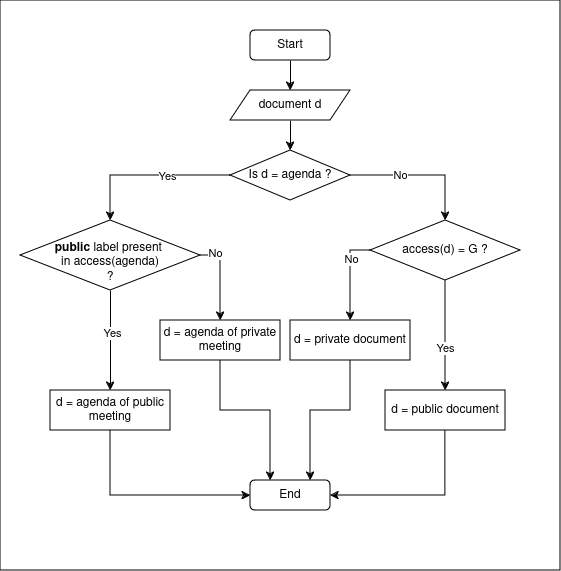
\includegraphics[width=0.8\textwidth]{./image/document_puclic_vs_private_classification.png}
    \caption{Process to identify whether a document is private or public}
    \label{fig:process to identify whether a document is private or public}
\end{figure} 

\noindent
Regarding other documents except agenda, for simplicity of implementation, we can include only \textbf{public} label in access control list, without including any other group of $\mathcal{G}$, to mean that $access(d) = \mathcal{G}$ or that document is a public document. Because, we do not need to include any other group ($g$) in a public non-agenda document, though we required them in public agenda documents for identifying meeting participants.\\ \\
\noindent
In addition to presence or absence of \textbf{public} label in $access(agenda)$, meeting agenda should define the \textbf{meeting quorum}, for the meeting. This theme will be discussed later.

% Definition of a meeting
\section{Definition of a meeting}

\noindent
\textbf{We assume that every meeting has an agenda associated with it, to define the set of groups($g$) required to attend the meeting}. Agenda of a particular meeting $M$ is a document, belonging to set $\mathcal{D}$.\\ \\
When we consider the agenda document of meeting $M$, for every group $g$ invited to meeting $M$; $g \in access(agenda)$. Also consider that, $D$ represents set of documents discussed in $M$, including agenda, such that $D \subseteq \mathcal{D}$. Hence, according to the assumption emphasized above, for any meeting $M$; $|D| \geq 1$.\\ \\ 
For conducting a meeting, at least 2 individuals are required. Consider that $I$ represents the set of individuals attending meeting $M$, such that $I \subseteq \mathcal{I}$, when groups ($g$) of $access(agenda)$ are converted to corresponding elementary individuals ($i$). Here we note that, for any meeting $M$; $|I| \geq 2$.\\
Accordingly, when $access(agenda)$ is defined in terms of singleton subsets of $\mathcal{G}$, and those groups (singleton subsets) in $access(agenda)$ are represented by $G$, such that $G \subseteq \mathcal{G}$, it can be observed that $|G| \geq 2$. \\ \\  
Consider set of locations of individuals in $M$ as $L$ (in other words, set of locations of individuals in set $I$, during meeting time), such that $L \subseteq \mathcal{L}$. Every individual attends meeting from a particular location $l$, such that $l \in L$. We note that, if meeting is online or hybrid, $|L| > 1$. If meeting is onsite, $|L| = 1$, since every individual is at same location. Every meeting should be in one mode, out of online, hybrid, onsite modes. Therefore, for any meeting $M$; $|L| \geq 1$. \\ \\
Since a \textbf{meeting} is a \textbf{synchronous} communication, every individual in meeting $M$ should attend the meeting during the same time slot $t$ (Assuming that all individuals are in same time zone).  \\ \\
Based on these definitions, we define meeting M as a 4-tuple,
    \[ M = < D, I, L, t > \]
such that,
    \[ D \subseteq \mathcal{D} \]
    \[ L \subseteq \mathcal{L} \]
    \[ I \subseteq \mathcal{I} \]
    \[ t \in \mathcal{T} \]


% Transformation of individual into role
\section{Transformation of individual into role}
\noindent
Consider that same sets defined above will be used in explanations below, in same notations: \\ \\
\noindent
Consider $g$ and $g'$ as subsets of $\mathcal{G}$ such that $g, g' \subseteq \mathcal{G}$. And consider $d$ as a \textbf{private} document , $l$ as a location and $t$ as a time slot such that $d \in \mathcal{D}$, $l \in \mathcal{L}$ and $t \in \mathcal{T}$.
Further consider that $g \in access(d)$ and $g' \notin access(d)$, for restricting access of document $d$, where $|access(d)| = n$ , given that $access(d)$ is defined as a set of singleton subsets of $\mathcal{G}$. A singleton subset of $\mathcal{G}$ means an elementary subset $g$, in which only one element (i.e. only one individual $i$) is present.\\ 
Also note that, $i$ and $i'$ are two individuals representing subsets $g$ and $g'$, respectively. \\ \\
\noindent
Assume that at scenario 1, $i$ attends a \textbf{meeting} at location $l$ during time slot $t$ to discuss document $d$, where $i'$ has no access to location $l$ during same time slot $t$. \\
Here we state that privacy of meeting discussing document $d$ was preserved at context $l \times t$ \\ \\ 
\noindent
Now assume that at scenario 2, $i$ attends a \textbf{meeting} at location $l$ during time slot $t$ to discuss document $d$, where $i'$ also has access to location $l$ during same time slot $t$. \\
Here we state that privacy of meeting discussing document $d$ was violated at context $l \times t$, because $n + 1$ individuals including $i'$ have got access to content of document $d$. But actually $|access(d)| = n$, when $access(d)$ is defined as a set of singleton subsets of $\mathcal{G}$, as mentioned above. We observe that $(n + 1) \geq |access(d)| = n$ \\ \\ 
\noindent
When above 2 scenarios are compared, we observe that role of same individual $i$, representing subset $g$ such that $g \in access(d)$, has experienced a variation. Context of $i$ has changed, depending on location and time. \\ \\
Therefore we define that presence of $i$ at context $l \times t$ transforms $i$ to role $r$.
\[ transform(i, l, t) = r : r \text{ is role of } i \text{ at location } l \text{ at time slot } t \] 
\noindent
If $g \in access(d)$, $g' \notin access(d)$ and $d$ is a \textbf{private} document, $i$ representing $g$ should attend a meeting to discuss $d$ at context $l \times t$, only if $i'$ representing $g'$ has no access to $l \times t$. Accordingly, to identify the privacy preserving context for discussing document $d$, combination of i, l, t is required.\\ \\



% Difference between public and private roles
\section{Difference between public and private roles}
When we consider a \textbf{private} document $d$, we can't exactly predict the time, at which $i'$, representing $g'$, such that $g' \notin access(d)$, will get access to location $l$. 
Therefore, meeting organizer has the responsibility of defining location $l$ as a \textbf{private} location or a \textbf{public} location, considering whether access of $i'$ has been strictly restricted, during all potential meeting time slots (represented by set $\mathcal{T}$).\\ \\
Using this definition and above formula, we can show that, $i$ representing $g$, such that $g \in access(d)$ where $d$ is a \textbf{private} document, is transformed to role $g$ itself, at a \textbf{private} location. 
Here, location should be defined as a \textbf{private} location, by same entity, that defined the set $access(d)$ for document $d$.

\[ transform(i, l, t) = r \]
\[ transform(i, (private\_location), t) = r \]
\[ transform(i, (private\_location), t) = g \] \\

\noindent
On the other hand, any location $l$ is defined as a \textbf{public} location, if access of $i'$ has \textbf{not} been strictly restricted, during any potential meeting time slot in set of time slots $\mathcal{T}$.\\ \\
Using this definition and above formula, we can show that, $i$ representing $g$, such that $g \in access(d)$, is transformed to \textbf{public} role, at a \textbf{public} location.
Location should be defined as a \textbf{public} location, by same entity, that defined the set $access(d)$ for document $d$.

\[ transform(i, l, t) = r \]
\[ transform(i, (public\_location), t) = r \]
\[ transform(i, (public\_location), t) = public \] \\
\noindent
Based on these derivations, we have identified a constraint relevant to $i$, for discussing $d$ in a privacy preserved meeting.\\ \\
\textbf{Constraint}: When $d$ is a \textbf{private} document, every $i$ representing $g$, such that $g \in access(d)$, that attends a meeting to discuss document $d$, must represent role $g$ in the meeting.\\ \\
When $d$ is a \textbf{public} document, every $i$ that attends a meeting to discuss document $d$, is allowed to represent \textbf{public} role in the meeting.\\ \\

% Sub-section: Roles in meeting agenda
\subsection{Roles in meeting agenda}
\noindent
If meeting agenda document does not include the group labeled as \textbf{public} in $access(agenda)$, it means that $\textbf{public} \notin access(agenda)$. Then $i'$ representing $g'$ such that $g' \notin access(d)$, should be strictly prevented from accessing the meeting, by conducting meeting at a \textbf{private} location, defined by relevant meeting organizing entity.\\ \\
On the other hand, if meeting agenda includes group labeled as \textbf{public} in $access(agenda)$, it means that $\textbf{public} \in access(agenda)$. Then it is \textbf{not} mandatory to prevent access of $i'$ representing $g'$ such that $g' \notin access(d)$, for the meeting. Therefore, meeting can be conducted at a \textbf{private} location or \textbf{public} location, based on locations defined by relevant meeting organizing entity.\\ \\

% Variation of role
\section{Variation of role}
\noindent
Now consider a situation where individual $i$ representing $g$, such that $g \in access(d)$ has $x$ number of locations, out of which any one can be selected for attending a meeting to discuss $d$. And assume that $i$ has $y$ number of time slots, out of which any one can be selected for attending the meeting.\\ \\
We can depict the possible variations of $transform(i, l, t)$ function as below, for individual $i$, depending on locations defined by the entity, assuming that $i$ doesn't change location during middle of a time slot.
\begin{table}[H]
    \centering
    \begin{tabular}{|c|c|c|c|c|c|}
    \hline
    $(i)$ & $t_1$ & $t_2$ & $...$ & $t_{y-1}$ & $t_{y}$ \\
    \hline
    $l_1$ & x & x & \  & x & x \\
    \hline
    $l_2$ & x & x & \  & x & x \\
    \hline
    $...$ & \  & \  & \  & \  & \  \\
    \hline
    $l_{x-1}$ & x & x & \  & x & x \\
    \hline
    $l_{x}$ & x & x & \  & x & x \\
    \hline
    \end{tabular}
    \caption{Possibilities in variation of $transform(i,l,t)$ for individual $i$}
    \label{tab:six_columns_six_rows}
\end{table}

\noindent
Note that $l_x$ represents the $x^{th}$ location, while $t_y$ represents the $y^{th}$ time slot. Meanwhile x represents the role of $i$ at the corresponding $l$ and $t$ (based on formula $transform(i, l, t) = r$). According to this representation, we observe that $i$ has $x \times y$ number of possibilities at maximum, to attain the role.\\ \\
Here we emphasize that some x roles can be categorized as \textbf{public}, with respect to \textbf{public} locations defined by an entity. According to the constraint identified, if $d$ is a \textbf{private} document, $i$ should attend the meeting only when $r = g$, such that $g \in access(d)$. When r = \textbf{public} role, individual $i$ should strictly avoid discussing \textbf{private} documents. By following this constraint, access of $i'$ representing $g'$, such that $g' \notin aceess(d)$, into this meeting can be prevented.\\ \\ 

% Meeting participant validation
\section{Privacy of documents}
\subsection{Participants in access control lists of non-agenda documents}
\noindent
It is possible to discuss one or more documents in a meeting. Further, there can be both public documents and private documents among these documents. We do not need to follow any constraint to protect the privacy of public documents.\\ \\
But when private documents are considered, it is needed to follow some constraints to protect the privacy. For example, consider $d_{1}$ and $d_{2}$ as 2 private documents. An individual $i$ representing $r$, such that $r = g$ and $g \in access(d_{1})$, can be absent in access control list of $d_{2}$. In other words, $g \notin access(d_{2})$ relationship can exist.\\ \\
In this situation, discussing both $d_{1}$ and $d_{2}$ in same meeting can violate the privacy of $d_{2}$, when above mentioned individual $i$ participates in that meeting. It means that, for discussing both $d_{1}$ and $d_{2}$ in same meeting, roles of all meeting participants should mandatorily be present in both $access(d_{1})$ and $access(d_{2})$. This relationship is graphically depicted in diagram below.
\begin{figure}[H]
    \centering
    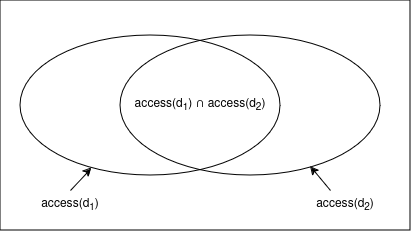
\includegraphics[width=0.7\textwidth]{./image/d1_intersection_d2.png}
    \caption{Intersection of access control lists of 2 private documents}
    \label{fig:intersection of access control lists of 2 private documents}
\end{figure} 
\noindent
This concept is applicable not only for 2 private documents, but also for any number of private documents discussed in same meeting. When there are $n$ number of private documents to discuss in a meeting, intersection of access control lists of all those documents should be considered. Any individual $i$ such that $i \notin (access(d_{1}) \cap access(d_{2}) \cap ... \cap access(d_{n-1}) \cap access(d_{n}))$ should be prevented from accessing the meeting.
\subsection{Meeting participant validation}
\noindent
When there are private documents to discuss in a meeting, it is required to validate intersection of participants identified as above, with participants included in access control list of meeting agenda (see "Meeting agenda" section for more details on meeting agenda).\\ 
For protecting privacy of $n$ number of private documents defined as $d_{1}, ... , d_{n}$, following relationship must be satisfied for the meeting. 
\[ access(agenda) \subseteq \{access(d_{1}) \cap access(d_{2}) \cap ... \cap access(d_{n-1}) \cap access(d_{n})\} \]
\noindent
Simply, above relationship means that each and every individual $i$ representing role $r$, such that $r = g$ and $g \in access(agenda)$, is also an element of the intersection of $access(d)$ of all private documents discussed in meeting.
A situation in which above relationship is violated can be explained by using following relationship. 
\[ \{access(d_{1}) \cap access(d_{2}) \cap ... \cap access(d_{n-1}) \cap access(d_{n})\} \subset access(agenda) \]
In simple terms, above relationship means that there exists at least one $i$ representing $r$, such that $r = g$ and $g \in access(agenda)$, where $g$ is not an element in the intersection of $access(d)$ of all private documents discussed in meeting.\\ \\
\noindent
However, for discussing public documents in meeting, it is not required to perform any participant validation. In other words, any individual $i$ can discuss public documents, in any private or public meeting.

% Privacy-preserved meeting
\section{Privacy-preserved meeting}
Based on above descriptions and definitions, we define privacy-preserved meeting as below;\\ \\
\textbf{A privacy-preserved meeting is a meeting in which, individual i representing role r has no access to the meeting, when $r = g$ and $g \notin access(agenda)$, where access(agenda) satisfies,} 
\[access(agenda) \subseteq \{access(d_{1}) \cap access(d_{2}) \cap ... \cap access(d_{n-1}) \cap access(d_{n})\} \]
\textbf{for all private documents $d_{1} ... d_{n}$, discussed in the meeting.} 

% Meeting quorum
\section{Meeting quorum}
\noindent
In a \textbf{privacy-preserved meeting} of our research context, we define \textbf{meeting quorum} as the minimum number of individuals ($i$) representing participant groups ($g$), required to attend a meeting, such that $g \in access(agenda)$. \\ \\
In privacy preserved meeting context, if a specific \textbf{meeting quorum} rule is not defined in the agenda, other than $access(agenda)$ set, we assume that every $i$ such that, 
\begin{itemize}
    \item $i \in g$, and
    \item $g \in access(agenda)$, 
\end{itemize}
\noindent
is required for the meeting. But, it is not applicable for $g = \textbf{public}$. In such a situation, when a numeric meeting quorum rule is not defined specifically, $|meeting\ quorum| = |access(agenda)|$, where $access(agenda)$ is defined in form of singleton subsets of $\mathcal{G}$. \\ \\
\noindent
In addition, it is possible that $|meeting\ quorum| < |access(agenda)|$, if a numeric \textbf{meeting quorum} rule is defined in meeting agenda. Therefore in overall, $|meeting\ quorum| \leq |access(agenda)|$, when $access(agenda)$ is defined in form of singleton subsets of $\mathcal{G}$. \\ \\
Since at least 2 individuals ($i$) are required for any meeting, $2 \leq |meeting\ quorum|$. \\ \\
Accordingly, $2 \leq |meeting\ quorum| \leq |access(agenda)|$. \\ \\
When $access(agenda)$ is defined in form of singleton subsets of $\mathcal{G}$, as we have already depicted earlier, $|access(agenda)| \leq |\mathcal{I}|$. By merging this inequality with above expression, we obtain following expression theoretically.\\ \\
$2 \leq |meeting\ quorum| \leq |access(agenda)| \leq |\mathcal{I}|$  \\ \\

% Problem analysis
\section{Problem analysis}
Our problem focused in organizing privacy-preserved meetings has few distinct steps, that can be clearly identified within it. Based on decision making points identified within the problem, this problem was mapped into a boolean circuit, following a union operation. Here, union operation can be introduced as a set related pre-processing operation, applied on the $access(d)$ sets of all documents of the meeting, including the $agenda$. Before applying this union operation, it is needed to make sure that, all groups except the $public$ group in those $access(d)$ sets are converted to singleton groups. Distinct sections of the problems are analyzed below, considering the circuit diagrams produced for them.\\ \\
% Participant validation based on documents
\subsection{Participant validation based on documents}
After calculating the union of $access(d)$ sets of all documents to be discussed in the meeting, as $access(doc\_1) \cap ... \cap access(doc\_n)\} \cap access(agenda)$, $public$ group is subtracted, since our initial requirement is to identify all the individuals having access to at least one document. In addition, we identify all documents associated with meeting as $doc\_1, ..., doc\_n, agenda$, since we need to check whether each individual in the union of individuals identified, has access to all the documents, for discussing them in a meeting. In example depicted in the diagram, consider that there are only 3 individuals as $i\_1, i\_2, i\_3$ and only 4 documents as $doc\_1, doc\_2, doc\_3, agenda$.\\ \\
Algorithm for participant validation section is explained below.
\begin{algorithm}[H]
    \caption{Participant validation based on documents}
    \begin{algorithmic}
        \State \textbf{Input:} Access control lists (access(d)) of documents \(doc\_1\), ... , \(doc\_n\), \(agenda\)
        \State \textbf{Output:} Eligibility of each individual for meeting by document analysis \\
        \State union of \(access(d)\) = \(access(doc\_1) \cup \dots \cup access(doc\_n) \cup access(agenda)\)
        \State union of individuals = union of \(access(d) - public \)
        \State set of documents = \(doc\_1, \dots , doc\_n , agenda\)
        \For{each \(i\_n\) in (union of individuals)}
            \State validity of \(i\_n\) by doc analysis = true
            \For{each \(doc\_x\) in (set of documents)}
                \If{\(doc\_x \neq agenda\)}
                    \State validity of \(i\_n\) for \(doc\_x\) = \((i\_n \in access(doc\_x)) \text{ OR } (public \in access(doc\_x))\)
                \Else
                    \State validity of \(i\_n\) for \(doc\_x\) = \(i\_n \in access(agenda)\)
                \EndIf
                \State validity of \(i\_n\) by doc analysis = validity of  \(i\_n\) by doc analysis \(\text{ AND validity of } i\_n\) for \(doc\_n\)
            \EndFor
            \State \textbf{Return} validity of \(i\_n\) by doc analysis
        \EndFor
    \end{algorithmic}
\end{algorithm}
Above algorithm explains the process depicted by logical circuit diagram below. In the algorithm, 
\[|union\ of\ access(d)| = |access(doc\_1)| + ... + |access(doc\_n)| + |access(agenda)| \]
relationship means that time complexity of the $union\ of\ access(d)$ operation is, $O(|access(doc\_1)| + ... + |access(doc\_n)| + |access(agenda)|)$. It is a linearly increasing time complexity. In addition, each iteration in outer loop outputs whether an individual of the union of individuals is valid by $access(d)$ analysis of all documents. Inner loop checks whether particular individual has access to all documents including $agenda$. Operations within the loops are considered as operations of constant time complexity, $O(1)$. Accordingly, since there is a nested loop in above algorithm, time complexity of this section of problem can be $O(n^{2})$, at maximum. Because number of individuals can be any positive integer, and number of documents including $agenda$ also can be any positive integer. 

\begin{figure}[H]
    \centering
    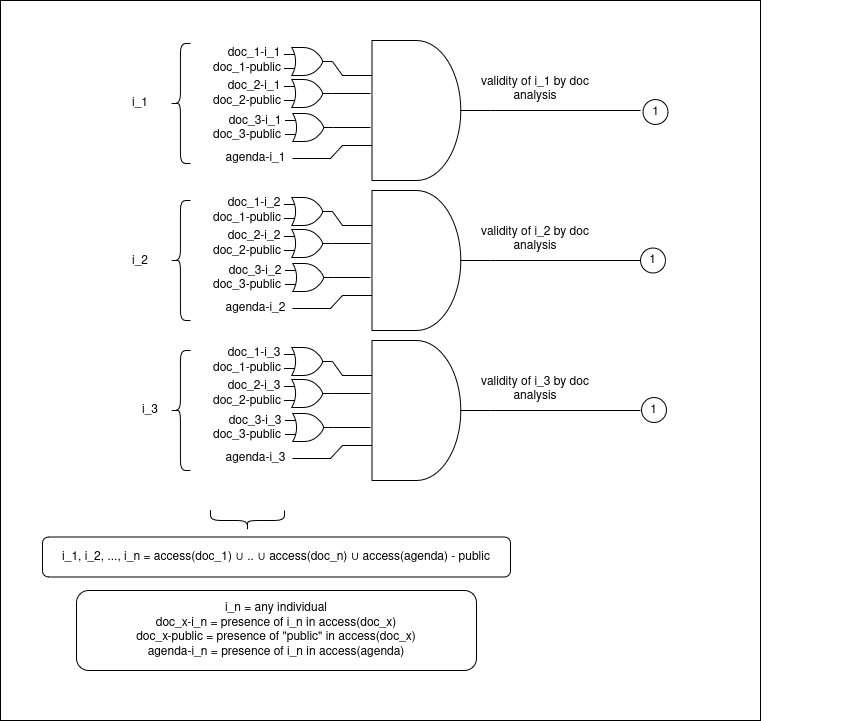
\includegraphics[width=0.9\textwidth]{./image/circuit_diagram/1_participant_validation.png}
    \caption{Participant validation based on $access(d)$ of documents}
    \label{fig:participant validation based on documents}
\end{figure} 

% Meeting quorum satisfiability of time slots
\subsection{Meeting quorum satisfiability of time slots}
\subsubsection{Eligibility of each individual, in each time slot, for meeting}
After checking the validity of each participant by document analysis, it is needed to check their locations in different time slots. Based on the location, eligibility of each individual to discuss the set of documents changes. Because, as we have described earlier, $private$ documents should be discussed at $private$ locations only, while $public$ documents can be discussed at any location. If there is at least one $private$ document in the set of documents discussed in meeting, then each individual $i\_n$ validated by document analysis should attend this meeting from a $private$ location. Following circuit diagram consists of the location analysis of each individual, in every time slot. Here, these time slots mean the time slots belonging to the union of available time slots of all individuals, present in the union of individuals, mentioned in previous algorithm.\\ \\ 
For deciding the eligibility of each individual, to discuss set of documents, in different time slots, we need inputs included in the following table. In it, each individual of the union of individuals, and his/her available time slots with locations should be present. Please note that following table consists of some sample data only, as individuals, time slots and locations. It is supposed to contain the real data, regarding the respective scenario. For simplicity, we consider only 3 locations as onsite, remote\_private and remote\_public, since every location can be categorized into one of those 3 categories, by a meeting organizing entity.\\ \\
\begin{table}[H]
    \centering
    \begin{tabular}{|c|c|c|}
    \hline
    Individual $(i\_x)$ & Time slot(slot$y$) & Location \\
    \hline
    $i\_1$ & slot1 & onsite \\
    \hline
    $i\_1$ & slot2 & remote\_private \\
    \hline
    $i\_1$ & slot3 & remote\_public \\
    \hline
    ... & ... & ... \\
    \hline
    $i\_n$ & slot$m$ & location of $i\_n$ in slot$m$ \\
    \hline
    \end{tabular}
    \caption{Available time slots and locations of individuals, in union of individuals}
    \label{tab:three_columns_six_rows}
\end{table}

Algorithm for deciding the eligibility of each individual, to discuss the set of documents of meeting, in different time slots, is described below.\\ \\
\begin{algorithm}[H]
    \caption{Deciding eligibility of each individual for meeting, in each time slot}
    \begin{algorithmic}
        \State \textbf{Input 1:} Validity of each individual \(i\_1\), ... , \(i\_n\) by doc analysis
        \State \textbf{Note:} Individuals \(i\_1\), ... , \(i\_n\) mean union of individuals of previous algorithm, and \textbf{input 1} is obtained from output of previous algorithm
        \State \textbf{Input 2:} Availability of each individual in each time slot (at any location) 
        \State \textbf{Input 3:} Location of each individual in each time slot (whether remote\_public or no)
        \State \textbf{Note:} \textbf{Input 2} and \textbf{input 3} are obtained from the table containing available time slots and locations of individuals.
        \State \textbf{Input 4:} Presence of \(public\) group in \(access(d)\) of each document, in set of documents, as $(doc\_1-public) , ... , (doc\_n-public) , (agenda-public)$
        \State \textbf{Output:} Eligibility of each individual, to discuss the set of documents, in each time slot \\
        \State union of time slots = \(availability(i\_1) \cup \dots \cup availability(i\_n)\)
        \For{each slot\(x\) in (union of time slots)}
            \For{each \(i\_y\) in (union of individuals)}
                \State publicity of meeting = \((doc\_1-public) \text{ AND } ... \text{ AND } (doc\_n-public) \text{ AND } (agenda-public)\)
                \State slot\(x-i\_y\) = availability of \(i\_y\) in slot\(x\) at any location
                \State slot\(x-i\_y\)\_remote\_public = whether \(i\_y\) is at remote\_public location in slot\(x\) 
                \State availability of slot\(x-i\_y\) for public meeting = (publicity of meeting) AND (slot\(x-i\_y\))
                \State availability of slot\(x-i\_y\) for private meeting = (slot\(x-i\_y\)) AND NOT(slot\(x-i\_y\)\_remote\_public)
                \State availability of slot\(x-i\_y\) for meeting by time slot analysis = (availability of slot\(x-i\_y\) for public meeting) OR (availability of slot\(x-i\_y\) for private meeting)
                \State slot\(x-i\_y\) eligibility for meeting = (Validity of \(i\_y\) by doc analysis) AND (availability of slot\(x-i\_y\) for meeting by time slot analysis)
            \EndFor
            \State \textbf{Return} slot\(x-i\_y\) eligibility for meeting
        \EndFor
    \end{algorithmic}
\end{algorithm}
In above algorithm, time complexity of $union\ of\ time\ slots$ operation is,\\ $O(|availability(i\_1)| + \dots + |availability(i\_n)|)$, at maximum. It is a linear time complexity. When considering the loops, outer loop iterates through all time slots, in the union of time slots, calculated by considering available time slots of all individuals, in union of individuals. Meanwhile, inner loop iterates through each individual in the union of individuals. In addition, number of documents discussed in the meeting can be any positive integer. Number of documents is considered when deciding the meeting publicity, within the inner loop. Further, validity of the individual by document analysis, obtained from output of previous algorithm, is utilized in in inner loop. Number of documents is concerned for that as well. But, it is in parallel level, with publicity calculation of the meeting. Therefore, we can consider that number of documents has linear time complexity as $O(n)$, within inner loop. Accordingly, it is observed that, time complexity of above algorithm can be $O(n^{3})$, at maximum, due to outer loop, inner loop, and number of documents within inner loop.\\ \\
Circuit diagram corresponding to above algorithm is depicted below. The following boolean circuit is supposed to be repeated for each individual, in each time slot, as explained in algorithm.
\begin{figure}[H]
    \centering
    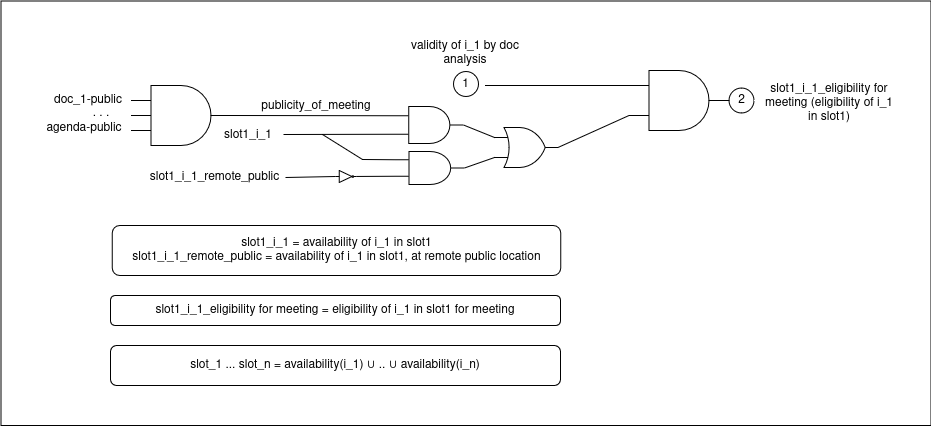
\includegraphics[width=0.9\textwidth]{./image/circuit_diagram/2_slot_n_i_n_eligibility.png}
    \caption{Eligibility of each individual for meeting, in each time slot}
    \label{fig:eligibility of each individual for meeting, in each time slot}
\end{figure} 

\subsubsection{Meeting quorum satisfiability}
Eligibility of each individual to discuss the set of documents, in each time slot, is considered for deciding the quorum satisfiability of each time slot, in the union of time slots. Then it is checked whether there is at least one quorum satisfying time slot. Because, if there is no at least one quorum satisfying time slot, then it is not possible to conduct the meeting.\\ \\
Algorithm for checking the quorum satisfiability of time slots is explained below.
\begin{algorithm}[H]
    \caption{Identifying meeting quorum satisfiability of time slots}
    \begin{algorithmic}
        \State \textbf{Input 1:} Eligibility of each individual for meeting, in each time slot
        \State \textbf{Note:} \textbf{Input 1} is obtained from output of previous algorithm
        \State \textbf{Input 2:} Numerical meeting quorum value 
        \State \textbf{Input 3:} Availability of each individual in each time slot (at any location)
        \State \textbf{Output:} Existence of quorum satisfying time slot/s, for the meeting \\
        \State union of time slots = \(availability(i\_1) \cup \dots \cup availability(i\_n)\)
        \State availability of a meeting quorum satisfying time slot = false
        \For{each slot\(x\) in (union of time slots)}
            \State meeting quorum satisfiability of slot\(x\) = false
            \State combinations of individuals in slot\(x\) = combinations of individuals, with magnitude of meeting quorum size 
            \For{each \(combination\) in (combinations of individuals in slot\(x\))}
                \State meeting quorum satisfiability of \(combination\) = AND operation (for all individuals in the \(combination\))
                \State meeting quorum satisfiability of slot\(x\) = (meeting quorum satisfiability of slot\(x\)) OR (meeting quorum satisfiability of \(combination\))
            \EndFor
            \State \textbf{Return} availability of a meeting quorum satisfying time slot = (availability of a meeting quorum satisfying time slot) OR (meeting quorum satisfiability of slot\(x\))
        \EndFor
    \end{algorithmic}
\end{algorithm}
Similar to previous algorithm, in above algorithm also, time complexity of $union\ of\ time\ slots$ operation is, $O(|availability(i\_1)| + \dots + |availability(i\_n)|)$, at maximum. It is observed that, in loop structure, outer loop iterates through all time slots in union of time slots. That number of time slots can be any positive integer. Inner loop contains a $combination$ operation, which is intended to create combinations of magnitude of meeting quorum size, out of individuals of the union of individuals. Mathematically, number of such possible combinations can be calculated as,
\[ n \text{C} r = \binom{n}{r} = \frac{n!}{r!(n-r)!} \]
when n = number of individuals in union of individuals, and r = meeting quorum size.\\ \\
Regarding $combination$ operation, highest number of combinations is obtained when $r = \frac{n}{2}$ or $r \approx \frac{n}{2}$. Number of possible combinations reduces, when $r$ is considerably small ($r \approx 1$), or when $r$ is approximately equal to $n$ ($r \approx n$). Due to this nature of $combination$ operation, maximum possible time complexity for creating $n \text{C} r$ number of combinations is $O(n \text{C} (n/2))$.\\ \\
In the inner loop of above algorithm, since AND operation is applied for all individuals, in each $combination$ created, maximum time complexity associated with inner loop is $O(n \text{ x } n \text{C} (n/2))$. Because, number of individuals in each combination created, or the meeting quorum size, can be any positive integer. In addition, since inner loop is repeated by outer loop, where number of time slots also can be any positive integer, maximum possible time complexity of above algorithm is, 
\[O(n \text{ x } n \text{ x } n \text{C} (n/2)) = O(n^{2} \text{ x } n \text{C} (n/2)) \]
Time complexity of $O(n^{2} \text{ x } n \text{C} (n/2))$ has polynomial component of $O(n^{2})$. Further, when considering $O(n \text{C} (n/2))$ component, it is observed that, for large $n$ values, 
\[ O(n \text{C} (n/2)) \approx O(2^{n}) \]
Time complexity of $O(2^{n})$ is considered as an exponential time complexity. Since exponential time complexity is non-polynomial (NP), it is eligible to use a heuristic or an existing library, when implementing above algorithm for execution with inputs. Because, there is no specific standard methodology defined, for creating combinations, as included in above algorithm.\\ \\
Figure below depicts the corresponding boolean circuit for above algorithm.\\ \\

\begin{figure}[H]
    \centering
    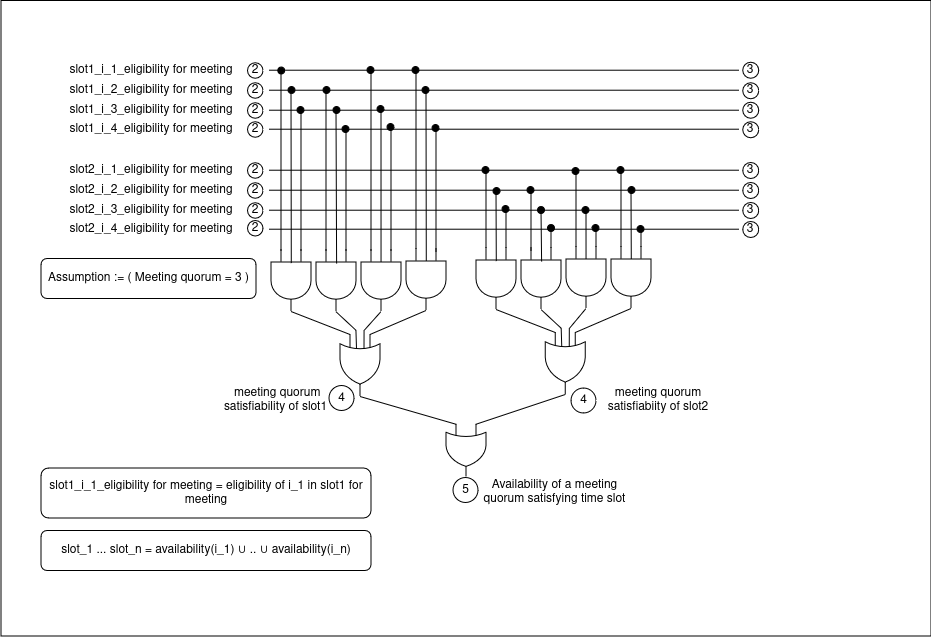
\includegraphics[width=0.9\textwidth]{./image/circuit_diagram/3_quorum_satisfying_slot_selection.png}
    \caption{Meeting quorum satisfiability of time slots}
    \label{fig:meeting quorum satisfiability of time slots}
\end{figure} 

% Earliest time slot selection
\subsection{Selection of earliest, meeting quorum satisfying time slot}
Selecting the earliest, meeting quorum satisfying time slot is not required to find a solution for our research problem. Because, after identifying the quorum satisfying time slots by above algorithm, our next objective associated with research problem is to, analyze the privacy-preserving meeting mode for each meeting quorum satisfying time slot. Therefore, we introduce this step of selecting the earliest, meeting quorum satisfying time slot, as an additional step provided by us. Since privacy-preserved meeting organization is a real world problem, when implementing a usable system for that purpose, this additional step can be helpful to identify the ealiest, eligible time slot for conducting the privacy-preserved meeting, rather than suggesting numerous eligible time slots.\\ \\
Algorithm for selecting the earliest, meeting quorum satisfying time slot is explained below.\\ \\
\begin{algorithm}[H]
    \caption{Selection of earliest, meeting quorum satisfying time slot}
    \begin{algorithmic}
        \State \textbf{Input:} Meeting quorum satisfiability of time slots, in union of time slots
        \State \textbf{Note:} \textbf{Input} is produced by processing previous algorithm
        \State \textbf{Output:} Earliest, meeting quorum satisfying time slot \\
        \State union of time slots with quorum satisfiability = quorum satisfiability of each time slot, in \((availability(i\_1) \cup \dots \cup availability(i\_n))\), in the order of precedence
        \State earliest eligible time slot = initialization of an empty list type structure, to store whether each slot is earliest eligible slot or no
        \For{each slot\(x\) and \(meeting\_quorum\_satisfiability\) in (union of time slots with quorum satisfiability)}
            \If{slot\(x\) is earliest slot in (union of time slots with quorum satisfiability)}
                \State store slot\(x\) and its \(meeting\_quorum\_satisfiability\), in (earliest eligible time slot) list     
            \Else
                \State previous condition = list to store result of, NOT operation (for each slot currently stored in (earliest eligible time slot) list)
                \State previous condition integrated = AND operation (for all slots in (previous condition) list) 
                \State whether slot\(x\) is earliest meeting quorum satisfying time slot = ((\(meeting\_quorum\_satisfiability\) of slot\(x\) = true) AND ((previous condition integrated) = true))
                \State store slot\(x\) and (whether slot\(x\) is earliest meeting quorum satisfying time slot), in (earliest eligible time slot) list                
            \EndIf
        \EndFor
        \State \textbf{Return} (earliest eligible time slot) list 
        \State \textbf{Note:} At \textbf{Return} point, (earliest eligible time slot) list contains \(true\) for earliest, meeting quorum satisfying time slot, and \(false\) for all other time slots
    \end{algorithmic}
\end{algorithm}

In above algorithm, there is a reason to apply a different process on the earliest time slot in union of time slots, apart from all other time slots in the union. If earliest time slot in union of time slots satisfies the meeting quorum, then without considering any pre-condition, it becomes the earliest meeting quorum satisfying time slot. It can be analyzed by extracting it as a separate condition, like below. \\ \\
\textbf{If} earliest slot in union of time slots satisfies the meeting quorum, \textbf{Then} \\
\indent earliest slot is the earliest, meeting quorum satisfying time slot \\
\textbf{Else}\\
\indent earliest slot is \textbf{not} the earliest, meeting quorum satisfying time slot \\
\textbf{EndIf}  \\ \\
Above condition block is the meaning implied by "If" block, in the condition of the algorithm. But, if any time slot other than the earliest time slot of union, satisfies the meetng quorum, then it is needed to check an additional condition as well, to identify whether it is the \textbf{earliest} meeting quorum satisfying time slot or no. Accordingly, following condition block elaborates the meaning implied by "Else" block of the condition, in above algorithm. \\ \\             
\textbf{If} any slot$x$ which is \textbf{not} the earliest slot in union of time slots, satisfies the meeting quorum, \textbf{Then} \\
\indent \textbf{If} any earlier slot than slot$x$ does \textbf{not} satisfy the meeting quorum, \textbf{Then} \\
\indent \indent slot$x$ is the earliest, meeting quorum satisfying time slot \\
\indent \textbf{EndIf}\\
\textbf{Else}\\
\indent slot$x$ is \textbf{not} the earliest, meeting quorum satisfying time slot \\
\textbf{EndIf}  \\ \\
It is observed that, there is a nested "If" condition in "If" block, in above condition block. Requirement to check this additional condition, is the reason for treating earliest time slot in union of time slots in a different manner, than other time slots, when identifying the earliest meeting quorum satisfying time slot.\\ \\
Above algorithm utilizes the meeting quorum satisfiability of each time slot, obtained by processing previous algorithm. Therefore, When we calculate the time complexity of above algorithm, we consider that meeting quorum satisfiability information is stored in an eligible data structure after processing previous algorithm. Otherwise, if we consider these both algorithms together, time complexity of above algorithm and previous algorithm collectively becomes, $O(2^{n})$ at maximum, as explained in time complexity description of previous algorithm.\\ \\
But, when meeting quorum satisfiability information obtained from previous algorithm is stored in an eligible data structure and provided to above algorithm, time complexity of above algorithm is dominated by "for" loop, and its content. Number of iteration in this loop can be any positive integer. There is no inner loop, in the "for" loop. But, in "Else" block of each iteration, "NOT" operation is applied on each time slot, until the slot which is currently being iterated by "for" loop. Therefore, it is observed that, time complexity of above algorithm can be $O(n^{2})$, at maximum. Even though there is an "AND" operation applied on all time slots, in the "Else" block, it can be neglected, when calculating time complexity. Because, it is in the parallel level to "NOT" operation, which is already considered. All other operations within above algorithm are considered as operations having constant time complexity.\\ \\
Circuit diagram corresponding to above algorithm is depicted below.\\ \\

\begin{figure}[H]
    \centering
    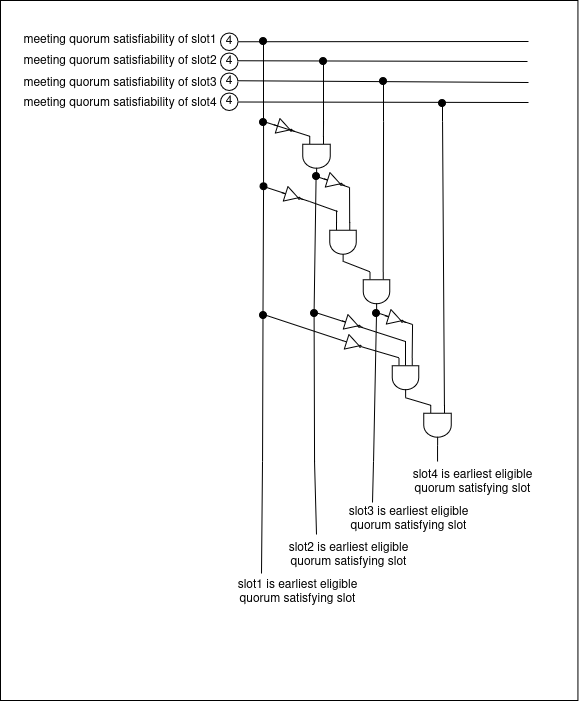
\includegraphics[width=0.9\textwidth]{./image/circuit_diagram/4_earliest_slot_selection.png}
    \caption{Selection of earliest, meeting quorum satisfying time slot}
    \label{fig:selecting earliest, meeting quorum satisfying time slot}
\end{figure} 

\end{document}

